\documentclass{beamer}
\usepackage[utf8]{inputenc}

\usetheme{Madrid}
\usecolortheme{default}
\usepackage{amsmath,amssymb,amsfonts,amsthm}
\usepackage{txfonts}
\usepackage{tkz-euclide}
\usepackage{listings}
\usepackage{adjustbox}
\usepackage{array}
\usepackage{tabularx}
\usepackage{gvv}
\usepackage{lmodern}
\usepackage{circuitikz}
\usepackage{tikz}
\usepackage{graphicx}

\setbeamertemplate{page number in head/foot}[totalframenumber]

\usepackage{tcolorbox}
\tcbuselibrary{minted,breakable,xparse,skins}



\definecolor{bg}{gray}{0.95}
\DeclareTCBListing{mintedbox}{O{}m!O{}}{%
  breakable=true,
  listing engine=minted,
  listing only,
  minted language=#2,
  minted style=default,
  minted options={%
    linenos,
    gobble=0,
    breaklines=true,
    breakafter=,,
    fontsize=\small,
    numbersep=8pt,
    #1},
  boxsep=0pt,
  left skip=0pt,
  right skip=0pt,
  left=25pt,
  right=0pt,
  top=3pt,
  bottom=3pt,
  arc=5pt,
  leftrule=0pt,
  rightrule=0pt,
  bottomrule=2pt,
  toprule=2pt,
  colback=bg,
  colframe=orange!70,
  enhanced,
  overlay={%
    \begin{tcbclipinterior}
    \fill[orange!20!white] (frame.south west) rectangle ([xshift=20pt]frame.north west);
    \end{tcbclipinterior}},
  #3,
}
\lstset{
    language=C,
    basicstyle=\ttfamily\small,
    keywordstyle=\color{blue},
    stringstyle=\color{orange},
    commentstyle=\color{green!60!black},
    numbers=left,
    numberstyle=\tiny\color{gray},
    breaklines=true,
    showstringspaces=false,
}
%------------------------------------------------------------

\title
{1.11.5}
\date{August 26,2025}
\author 
{AI25BTECH11003 - Bhavesh Gaikwad}



\begin{document}


\frame{\titlepage}
\begin{frame}{Question}
The scalar product of vector $\overrightarrow{a} = \hat{i} + \hat{j} + \hat{k}$ with a unit vector along the sum of the vectors $\overrightarrow{b} =2\hat{i} + 4\hat{j} - 5\hat{k} $ and $\overrightarrow{c} = \lambda\hat{i} + 2\hat{j} + 3\hat{k}$ is equal to 1. Find the value of $\lambda$ and hence find the unit vector along $\overrightarrow{b} + \overrightarrow{c}$.
\end{frame}


\begin{frame}[fragile]
    \frametitle{Theoretical Solution}
 Given: $\vec{a}=\myvec{1\\1\\1}$,  $\vec{b}=\myvec{2\\4\\-5}$,  $\vec{c}=\myvec{\lambda\\2\\3}.$

Let $\vec{u}$ be the unit vector along $\vec{b} + \vec{c} .$ \\

$ \vec{b} + \vec{c} = \myvec{2+\lambda\\4+2\\-5+3}
=\myvec{2+\lambda\\6\\-2}.$ \\

$\|\vec{b}+\vec{c}\| = \sqrt{(2+\lambda)^2+6^2+(-2)^2}
 = \sqrt{\lambda^2+4\lambda+44}.$ \\

$\vec{u}$ = $\dfrac{\vec{b} + \vec{c}}{\|\vec{b}+\vec{c}\|}$ = $\dfrac{1}{\sqrt{\lambda^2+4\lambda+44}} \myvec{2+\lambda\\6\\-2}.$ 

\end{frame}


\begin{frame}[fragile]
    \frametitle{Theoretical Solution}
    Given condition: $\vec{a}\cdot \vec{u}=1.$  

$$ \vec{a}\cdot\vec{u} = \dfrac{\vec{a}\cdot(\vec{b}+\vec{c})}{\|\vec{b}+\vec{c}\|}
= \dfrac{\myvec{1\\1\\1}\cdot\myvec{2+\lambda\\6\\-2}}
{\sqrt{\lambda^2+4\lambda+44}}
= \dfrac{\lambda+6}{\sqrt{\lambda^2+4\lambda+44}}=1.
$$ \\


$
\Rightarrow\ (\lambda+6)^2=\lambda^2+4\lambda+44
\ \Longrightarrow\ 
\lambda^2+12\lambda+36=\lambda^2+4\lambda+44
\ \Longrightarrow\ 
8\lambda=8\ $
$$\Longrightarrow\ 
\boxed{\lambda=1}$$

Now, with $\lambda=1:\quad \vec{b}+\vec{c}
=\myvec{3\\6\\-2},\quad \|\vec{b}+\vec{c}\|
=\sqrt{3^2+6^2+(-2)^2} = \sqrt{49} = 7.$ \\
\end{frame}


\begin{frame}[fragile]
    \frametitle{Theoretical Solution}
Unit vector along, $\vec{b}+\vec{c}$ is: $\quad \dfrac{1}{7}\myvec{3\\6\\-2}
= \dfrac{1}{7}\myvec{3\\6\\-2}.$\\\\
\bigskip
\begin{align}   
\centering
\boxed{\lambda=1} \quad and \qquad 
\boxed{\text{Unit vector along }\,\vec{b}+\vec{c}
=\dfrac{1}{7}\myvec{3\\6\\-2}}.
\end{align}
\end{frame}


\begin{frame}[fragile]
    \frametitle{C Code}
    \begin{lstlisting}
#include <stdio.h>
#include <math.h>

#define DIM 3


void add(const double u[DIM], const double v[DIM], double out[DIM]) {
    for (int i = 0; i < DIM; ++i) out[i] = u[i] + v[i];
}

double dot(const double u[DIM], const double v[DIM]) {
    double s = 0.0;
    for (int i = 0; i < DIM; ++i) s += u[i] * v[i];
    return s;
}
    \end{lstlisting}
\end{frame}


\begin{frame}[fragile]
    \frametitle{C Code}
    \begin{lstlisting}
double norm(const double u[DIM]) {
    return sqrt(dot(u, u));
}

void scale(const double u[DIM], double s, double out[DIM]) {
    for (int i = 0; i < DIM; ++i) out[i] = s * u[i];
}

void normalize(const double u[DIM], double out[DIM]) {
    double n = norm(u);
    if (n == 0.0) {
         
        for (int i = 0; i < DIM; ++i) out[i] = 0.0;
    } else {
        scale(u, 1.0 / n, out);
    }
}
    \end{lstlisting}
\end{frame}


\begin{frame}[fragile]
    \frametitle{C Code}
    \begin{lstlisting}
int main(void) {
    
    const double a[DIM] = {1.0, 1.0, 1.0};
    const double b[DIM] = {2.0, 4.0, -5.0};

    
    const double lambda = 1.0;
    const double c[DIM] = {lambda, 2.0, 3.0};

    
    double s[DIM];
    add(b, c, s);            // s = (3, 6, -2)

    
    double uhat[DIM];
    normalize(s, uhat);      // uhat = (3/7, 6/7, -2/7)

    

    \end{lstlisting}
\end{frame}


\begin{frame}[fragile]
    \frametitle{C Code}
    \begin{lstlisting}

    printf("lambda = %.0f\n", lambda);
    printf("b + c = (%.2f, %.2f, %.2f)\n", s[0], s[1], s[2]);
    printf("||b + c|| = %.2f\n", norm(s));
    printf("Unit vector along (b + c) is: (%.2f, %.2f, %.2f)\n", uhat[0], uhat[1], uhat[2]);

    
    double check = dot(a, uhat);
    printf("Verification a * u = %.2f\n", check);

    return 0;
}
    \end{lstlisting}
\end{frame}


\begin{frame}[fragile]
    \frametitle{Python Code}
    \begin{lstlisting}

import numpy as np
import matplotlib.pyplot as plt

# Define vectors
a = np.array([1, 1, 1])
b = np.array([2, 4, -5])
lambda_val = 1
c = np.array([lambda_val, 2, 3])

# b + c and its unit vector
bc = b + c
bc_unit = bc / np.linalg.norm(bc)

\end{lstlisting}
\end{frame}

\begin{frame}[fragile]
    \frametitle{Python Code}
    \begin{lstlisting}
# Set up 3D plot
fig = plt.figure(figsize=(7, 7))
ax = fig.add_subplot(111, projection='3d')
ax.set_xlim([-1, 7])
ax.set_ylim([-1, 7])
ax.set_zlim([-6, 4])

# Origin
origin = np.zeros(3)

def plot_vec(ax, v, color, label):
    ax.quiver(*origin, *v, color=color, arrow_length_ratio=0.1, linewidth=2)
    ax.text(*(v*1.12), label, color=color, fontsize=13)
  
    \end{lstlisting}
\end{frame}


\begin{frame}[fragile]
    \frametitle{Python Code}
    \begin{lstlisting}
    
plot_vec(ax, a, 'blue', 'a')
plot_vec(ax, b, 'orange', 'b')
plot_vec(ax, c, 'green', 'c')
plot_vec(ax, bc_unit, 'red', '(b+c)/|b+c|')

# Labels and style
ax.set_xlabel('X')
ax.set_ylabel('Y')
ax.set_zlabel('Z')
ax.set_title('Vectors a, b, c and unit vector along (b+c)')
plt.tight_layout()

# Save the figure
plt.savefig('fig1.png')
plt.close()  

    \end{lstlisting}
\end{frame}


\begin{frame}{Vector Representation}
   \centering
    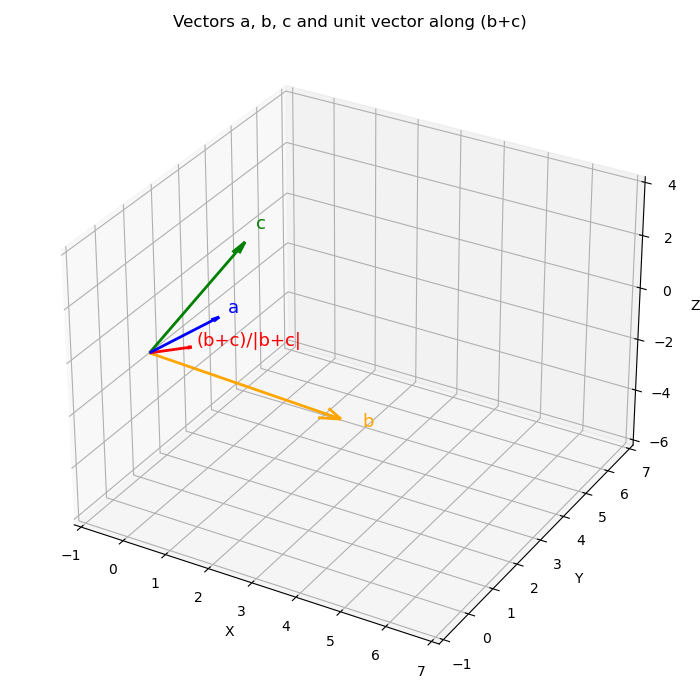
\includegraphics[width=\columnwidth, height=0.8\textheight, keepaspectratio]{figs/fig1.png}
    \label{fig:Beamer/figs/fig1.png}
\end{frame}


\end{document}